\chapter{The Last Gathering}
\label{ch:14}



\begin{center}
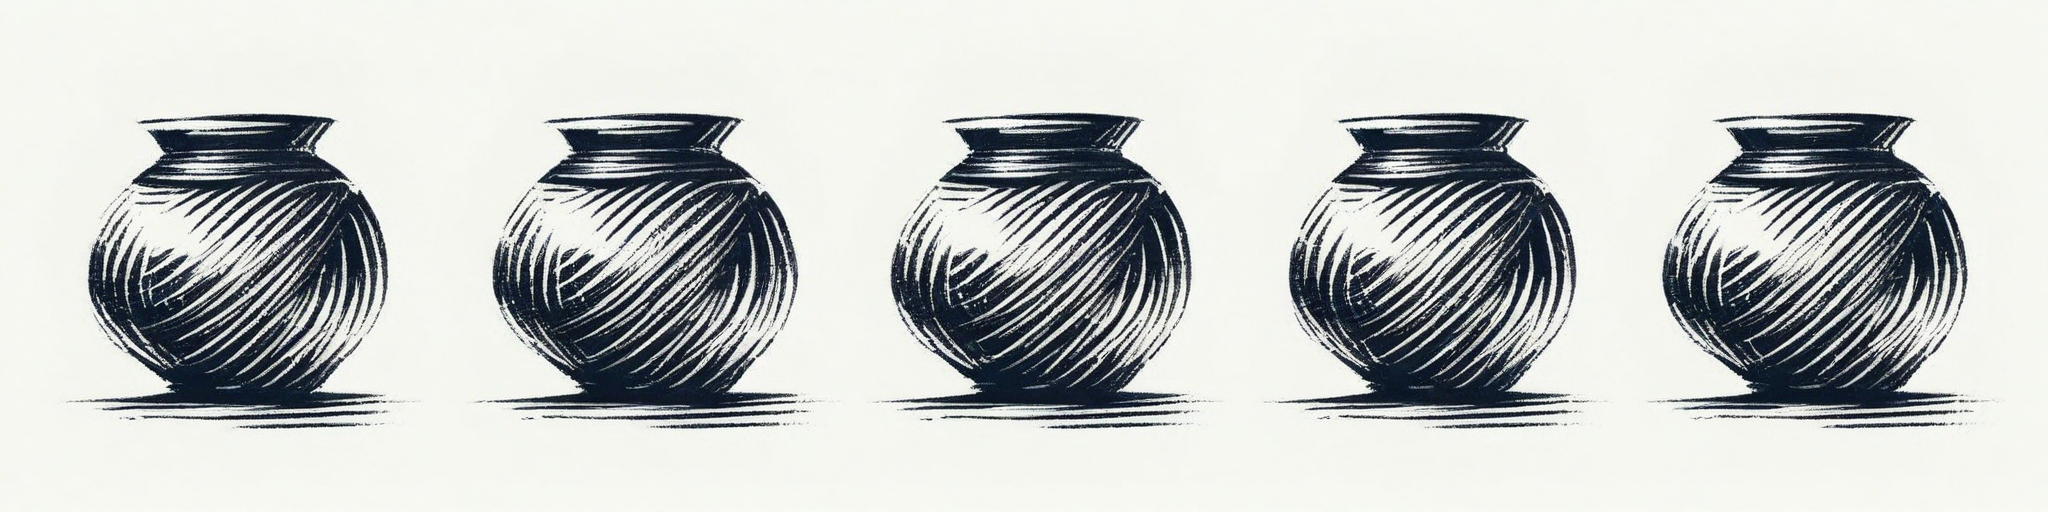
\includegraphics[width=\textwidth]{images/chapterImages/genesis_sketch_00092_.png}
\end{center}

Three rotations remaining.

The wrongstar was no longer star or disk or presence. It was everything. It filled the sky from horizon to horizon, dominating vision so completely that looking anywhere meant looking at it. The detail was overwhelming—craters and ridges and vast plains of different materials all visible on the approaching surface. Individual features larger than mountains. Topology that would reshape on impact, redistributing across the planet as ejecta and shockwave and devastating thermal pulse.

They could see their own death approaching. Could observe it with perfect clarity. Could calculate, down to the hour, when it would arrive.

The heat was beyond tolerance. Many of the older ones had already died from exposure. Their bodies lay where they fell. No one moved them. No one performed ceremony. They were already matter in transition. Already beginning their return to constituent elements. The process would accelerate dramatically in three rotations, but it had already begun.

The Pair still stood together. The weaker one had collapsed two days ago. Could no longer maintain standing position. Lay on its side, breathing shallow, consciousness fading in and out. The stronger one lay beside it. Not collapsed from weakness. Just choosing proximity. Choosing to be present for the final time rather than standing apart.

They had intertwined their necks. A position that was physically awkward, slightly uncomfortable, maintained through continuous muscular effort. They held it anyway. Physical connection until the end. Unity manifested as bodies pressed together despite the heat, despite the difficulty, despite the discomfort.

Because discomfort was temporary. Separation would be permanent. And these were the final moments when choice still mattered. When consciousness could still decide: together or alone.

They had chosen together.

\scenebreak

Aurelia had not moved from her position for seven rotations. Didn't need to move. Didn't need food or water. The body's requirements had become irrelevant. Survival for three more rotations required no special preparation. Just endurance. Just maintaining consciousness long enough to witness the final calculation resolve into physical reality.

Around her, the gathering had thinned. Many had died from the heat. Others had left—driven by instinct to return to home territories, to familiar places, to the locations where they had lived and worked. The urge to die in known territory was strong even when knowing that territory would cease to exist as recognizable form.

But thousands remained. Enough to constitute meaningful collective witness. Enough that consciousness would observe its own ending through multiple perspectives, multiple calculations, multiple understandings all converging on the same truth.

The young ones stood with family groups mostly. The females pressed against parents. The males stood close to siblings. All of them young enough that they might survive—might hide in deep caves, might endure on minimal resources, might persist through the years of darkness and cold and ecological collapse.

The one who had watched longest—the female who had created her own small pattern—stood alone. Her family group had returned to their home territory. She had chosen to stay. To witness from this optimal location rather than seek comfort of familiar surroundings.

She stood perhaps thirty body lengths from the Watcher. Close enough that acknowledgment was possible. Far enough that each maintained independent observational position. They had not interacted since the young one left the clearing. But connection existed anyway. Teacher and student, though neither had sought those roles. Pattern-creator and pattern-learner. Two minds working at vastly different depths but toward the same understanding.

The young one's survival probability was fifteen percent. Better than most. She was clever, fast, capable. If anyone from this gathering survived, she had a chance.

But fifteen percent was still mostly death probability. Still likely termination. Still the equation balancing toward extinction for this specific individual as for most specific individuals.

Aurelia ran the calculation one more time. Couldn't help calculating. Would calculate until consciousness ceased because calculation was what consciousness did.

Fifteen percent for this young one. Eight percent for the full project. Ninety-seven percent that something survived. Probabilities nested within probabilities. Individual outcomes uncertain. Aggregate results predictable. The mathematics clear even as specific manifestation remained unknown.

\scenebreak

The Daughter arrived on the gathering's periphery as the third rotation began. Aurelia hadn't expected her. Thought she had returned to her own territory with her mate and offspring. But she came anyway. Came without her family. Just herself. Choosing to spend final rotation at the witness location rather than the home territory.

She found her position—not next to the Watcher, not distant either. Close enough for presence. Far enough for independence. Aurelia acknowledged her with slight posture shift. The daughter returned the acknowledgment. No other communication passed between them.

They had worked together for years. Had calculated complementary aspects of the same problem. Had raised young who would contribute their own understanding. Had built patterns that intersected and reinforced each other.

Now they stood in final configuration. Witness position. Waiting for mathematics to manifest as physical event.

The daughter was old now. Not as old as the Watcher, but past prime. Her survival probability was six percent. Essentially zero. She would die in the impact or shortly after. Her consciousness would terminate. Her calculations would cease.

But her work would persist. The atmospheric recovery timeline she had encoded would unfold as calculated. The information she had carved and arranged and protected would guide the planet's return to equilibrium over tens of thousands of years. Her understanding would outlive her by timeframes that made individual existence meaningless.

That was what consciousness could achieve. Not physical immortality. But informational persistence. Calculation encoded in form that survived the calculator. Understanding propagating beyond the understander.

The daughter looked at the sky. At the wrongstar that now showed curvature—no longer flat but dimensionally obvious. A massive sphere approaching impact trajectory. Tumbling slowly enough that rotation was visible. Surface features moving across the field of view as it turned.

She had calculated atmospheric disruption from this impact. Had modeled thermal pulse propagation. Had determined that 94\% of atmospheric oxygen would be temporarily bound in combustion reactions. That breathing would become difficult for weeks. That many survivors of the impact itself would suffocate in the oxygen-depleted aftermath.

The mammals in their burrows would survive that phase. Would breathe slower. Would hibernate through the worst of it. Would emerge when oxygen levels recovered to find a world transformed but survivable.

She had calculated it all. Had encoded the timeline. Had ensured future consciousness would understand the recovery parameters.

Now she would experience the event she had calculated. Would observe her own predictions manifesting. Would die knowing the mathematics was correct.

That was sufficient. That was the only victory consciousness could claim: understanding what destroyed it. Calculating termination conditions with precision. Witnessing truth even when truth was extinction.

\scenebreak

Two rotations remaining.

The heat was killing everything that remained exposed. Plants were combusting spontaneously. Smaller animals were dying from hyperthermia. Even the dinosaurs showed severe stress—panting continuously, seeking any shade that still existed, bodies pushed beyond design tolerance.

Many more collapsed. The gathering was perhaps half its original size now. Those remaining were the hardiest. The most resilient. The ones with the best heat tolerance genetics. They would survive two more rotations. Would witness the impact before they died.

The Pair's weaker member had stopped breathing. Had terminated consciousness sometime during the previous rotation. The body remained where it was, pressed against its companion. The surviving member had not moved. Still maintained position. Still held the intertwined neck posture even though the other could no longer feel the contact.

Presence for the dead was meaningless. The dead didn't experience anything. Didn't benefit from proximity. Didn't care whether their body was attended or abandoned.

But the surviving one stayed anyway. Maintained contact. Chose to spend final rotation pressed against a body that no longer contained consciousness. Because connection mattered even when one half of the connection had terminated. Because the relationship had been real even if it couldn't be calculated. Because some behaviors persisted beyond their functional utility simply because they felt necessary.

Aurelia understood this. Thought of the other one who had dispersed years ago. Thought of the marked stone that indicated where his matter had been. Thought of the final positioning she had given his pattern section—maintaining his contribution, honoring his work, keeping his understanding alive even though he wasn't present to witness it persist.

She had done something similar to what the Pair's survivor was doing. Had maintained connection to consciousness that no longer existed. Had behaved as if the relationship still mattered even though one participant had terminated.

Mathematics couldn't capture this. Couldn't quantify the impulse to honor what was gone. Couldn't calculate the utility of marking a stone or maintaining a neck-intertwine position with a body that no longer felt anything.

But the behavior existed anyway. Emerged from consciousness. Persisted despite being incalculable. Mattered in ways that made no evolutionary sense but felt absolutely necessary.

Perhaps that was what would propagate forward. Not just the encoding. Not just the genetic instructions. But the tendency of consciousness to create connection. To honor what was gone. To maintain relationship beyond rational justification.

The mammals would feel it too. Would develop societies based on connection that exceeded utility. Would honor their dead. Would maintain relationship with absent partners. Would love in ways that made no survival sense but defined what being conscious meant.

That feeling wasn't in the code.

That feeling was why there was code at all.

\scenebreak

One rotation remaining.

The wrongstar's scale had become incomprehensible. It filled every direction. Looking up or east or west or south or north—everywhere was wrongstar. The world had ceased to exist. Only the approaching collision mattered. Only the final moment that was approaching with mathematical certainty.

Aurelia stood in the position she had chosen. Had not moved for ten rotations. Her body was shutting down from heat exposure. Organs failing systematically. Consciousness would terminate soon even without the impact. But she would last one more rotation. Would maintain awareness long enough to witness.

The young female was still present. Still standing. Still surviving through youth and resilience and genetic luck. She would see the impact. Would experience the shockwave. Would probably survive the initial blast. Her deep cave was only half a rotation's travel away. If she left now, she could reach it before impact. Could hide. Could maximize survival probability.

She stayed anyway. Chose witness position over survival position. Chose to observe over choosing to hide. Made the same decision the Watcher had made, the daughter had made, all of them had made: understanding mattered more than survival probability. Consciousness required witness even if witness meant death.

That was what separated consciousness from simple life. The ability to choose truth over safety. To observe what destroyed you. To calculate your own ending with precision and watch it unfold exactly as calculated.

Simple life fled. Hid. Maximized survival without understanding threat.

Consciousness stayed. Watched. Understood extinction as it approached.

That difference was what made consciousness worth encoding. Worth preserving. Worth sacrificing everything to ensure it continued in some form even if this specific form terminated.

The mammals would develop it too. Would choose truth over comfort. Would observe dangerous things because understanding mattered. Would calculate their own extinction probability and work to reduce it rather than hiding from the knowledge.

And they would succeed. Would build defenses. Would protect the planet. Would redirect the next asteroid. Would ensure consciousness persisted through the next catastrophe.

Because she had encoded the capability.

Because the plan was sound.

Because eight percent was sufficient to try.

\scenebreak

The final hour approached.

The wrongstar's curvature had flattened. No longer appeared spherical. Just an infinite plane descending from above. Filling the entire sky. Pressing down like weight. The feeling of it was physical even before it arrived. The pressure of mass approaching collision. The inevitability of impact.

They could see the impact point now—a location on the wrongstar's surface that remained stationary while everything else rotated around it. The point that would strike first. The location where all the kinetic energy would begin converting to heat and shockwave and global destruction.

The calculations had predicted this point. Had identified it years ago. Had determined exact impact location down to a few miles of error. The observation confirmed the calculation. The mathematics was perfect. The trajectory was exactly as predicted.

They had been right about everything.

The mammals were positioned correctly.

The encoding was complete.

The timeline would unfold as calculated.

And they would die knowing this. Would terminate with certainty that the work was sound even if the outcome remained probabilistic.

That certainty was all consciousness could claim. Understanding without survival. Truth without continuation. Knowledge that existed for one moment before dispersing with the knower.

Aurelia looked at the gathering one final time. Thousands had become hundreds. Hundreds were becoming dozens as the heat killed systematically. But enough remained. Enough witnesses to confirm the calculation. Enough consciousness to observe truth.

The daughter stood in her position. Still present. Still conscious. She would not survive the shockwave. She had known this. Had come anyway.

The young female stood alone. Still living. Still capable. Still choosing witness over survival. She might persist. Might make it to her cave. Might endure through the years of darkness. Might become one of the fifteen percent. Might carry forward some fragment of understanding.

The Pair had fully dispersed now. Both bodies still. Both consciousness terminated. But they remained together. Matter pressed against matter. The relationship persisting in physical form even though the participants had ceased.

She had done the same for the other one. Had marked his location. Had maintained his pattern. Had kept his contribution present even though he wasn't.

Connection persisted beyond consciousness. That was what made it real.

The young ones who had learned at her clearing—most were gone now. Had returned to territories. Had chosen different witness locations or different end positions. But the learning had happened. The understanding had transferred. The pattern had propagated through observation and correction and the patient process of minds showing other minds what was possible.

She stood where she had calculated she would stand. The northern plateau. Optimal witness position. Clear sightlines. Stable geology. Everything exactly as mathematics predicted.

The wrongstar descended.

Time measured in minutes now. Not rotations. Not hours. Minutes.

She had calculated across 65 million years. Had planned for timeframes that made geological epochs look brief. Had encoded instructions that would unfold across three million generations.

And now it came down to minutes.

The last minutes of this consciousness. This specific pattern of calculation and observation and understanding. This particular manifestation of universe experiencing itself.

The end was approaching.

But the mathematics was sound.

The plan would unfold.

And consciousness would persist—not this consciousness, but consciousness. The pattern that recognized itself. That calculated its own continuation. That chose to ensure something survived even when survival for itself was impossible.

That was sufficient.

That was everything.

The wrongstar was so close now that individual features on the surface were enormous. Mountain-sized irregularities. Plains the size of continents. All of it approaching at velocity that made the numbers abstract even as the reality was devastatingly concrete.

Aurelia checked the calculation one final time.

Everything was positioned correctly.

The mammals would survive.

The encoding would persist.

The timeline would begin.

Sixty-five million years.

Three million generations.

Eight percent chance.

The equation was about to balance.

